%! Author = Daniil
%! Date = 15.05.25

\documentclass[12pt]{article}
\usepackage{pdflscape}
\usepackage{rotating}
\usepackage{hyperref} % otočení tabulky

% +-------------------+
% | Rozložení stránek |
% +-------------------+
\usepackage[
    a4paper,
    width=150mm,
%  height=220mm,
    top=25mm,
    bottom=25mm
]{geometry}


% +------+
% | Font |
% +------+
\usepackage{fontspec}
\setmainfont{Linux Libertine O}


% +---------+
% | Čeština |
% +---------+
\usepackage[czech]{babel}


% +------------------------------------+
% | programovací jazyk Lua - LuaLaTeX  |
% +------------------------------------+
\usepackage{luacode}
\newcommand{\luavar}[1]{\directlua{tex.sprint(#1)}}
\begin{luacode*}
-- vrací uživatelem zadané datum nebo aktuální datum
function get_date()
  if (date == nill or date == '') then
    return tex.print('\\today')
  else
    return tex.print(date)
  end
end

-- vrací všechny autory dokumentu( jméno + obor) naformátované pro TeX
function get_authors()
  local result = ""
  for i, author in ipairs(authors) do
    result = result .. author.name .. "&&&&&" .. author.program .. "\\\\"
  end
  return result
end

-- vrací počet autorů
function get_authors_count()
    local result = 0
    for i, author in ipairs(authors) do
        result = result + 1
    end
    return result
end

-- vrací jména všech autorů oddělená čárkami
function get_author_names()
    local result = ""
    if get_authors_count() == 1 then
        return authors[1].name
    else
        for i, author in ipairs(authors) do
            result = result .. author.name .. ", "
        end
        result = result:sub(1, -3)
        return result
    end
end

-- podmíněné výpisy
function printBiblio()
  local output = "\\newpage \\section{Literatura} \\printbibliography[heading=none]"
  if (PRINT_BIBLIO) then
    return tex.print(output)
  end
end

function printTablesList()
    if (PRINT_TABLES) then
        return tex.print("\\listoftables")
    end
end

function printFiguresList()
    if (PRINT_FIGURES) then
        return tex.print("\\listoffigures")
    end
end

function printSnippetsList()
    if (PRINT_SNIPPETS) then
        return tex.print("\\lstlistoflistings")
    end
end
\end{luacode*}


% +---------+
% | seznamy |
% +---------+
\usepackage{multicol} % vícesloupcový seznam


% +---------+
% | chemie  |
% +---------+
\usepackage{chemformula}


% +---------+
% | obrázky |
% +---------+
\usepackage{graphicx}
\graphicspath{{./images/}}
\usepackage{svg}
\usepackage{subcaption}
\usepackage{wrapfig}


% +-------+
% | barvy |
% +-------+
\usepackage{color}
\definecolor{dkgreen}{rgb}{0,0.6,0}


% +--------+
% | odkazy |
% +--------+
\usepackage{hyperref}
\hypersetup{
    colorlinks=true,
    citecolor=black,
    filecolor=black,
    linkcolor=black,
    pdftitle={\luavar{title}},
    urlcolor=teal
}

% +------------------------------+
% |         bibliografie         |
% +------------------------------+
% | používá se norma ČSN ISO 690 |
% +------------------------------+
\usepackage{csquotes}
\usepackage[style=iso-authoryear,
    hyperref=true,
    url=false,
    isbn=false,
    backref=true]{biblatex}
\addbibresource{biblio.bib}
% převedení bibliografie do kapitálek
%\renewcommand{\mkbibcompletename}[1]{\textsc{#1}}  % afektuje kromě bibliografie i citace
\renewcommand*{\mkbibnamegiven}[1]{\textsc{#1}}


% +-----------------------+
% | sazba zdrojových kódů |
% +-----------------------+
\usepackage{listings}
\renewcommand{\lstlistingname}{Zdrojový kód}
\renewcommand{\lstlistlistingname}{Seznam zdrojových kódů}

% čeština ve zdrojovém kódu
\lstset{extendedchars}
\begingroup
\catcode0=12 %
\makeatletter
\g@addto@macro\lst@DefEC{%
    \lst@CCECUse\lst@ProcessLetter
    ěščřžĚŠČŘŽťŤďĎňŇů
    ^^00%
}%
\endgroup

% stylování zdrojového kódu (barvy klíčových slov, ...)
\lstdefinestyle{mystyle}{
    backgroundcolor=\color{white},
    commentstyle=\color{dkgreen},
    keywordstyle=\color{orange},
    numberstyle=\tiny\color{gray},
    stringstyle=\color{purple},
    basicstyle=\ttfamily\footnotesize,
    breakatwhitespace=false,
    breaklines=true,
    captionpos=b,
    keepspaces=true,
    numbers=left,
    numbersep=5pt,
    showspaces=false,
    showstringspaces=false,
    showtabs=false,
    tabsize=2
}
\lstset{style=mystyle}


% +--------------------------+
% | záhlaví a zápatí stránek |
% +--------------------------+
\usepackage{fancyhdr}


% +----------------------------+
% | vlastní použitelné příkazy |
% +----------------------------+
\newcommand\lorem{
    Lorem ipsum dolor sit amet, consectetur adipiscing elit, sed do eiusmod tempor incididunt ut labore et dolore magna aliqua. Ut enim ad minim veniam, quis nostrum exercitationem ullam corporis suscipit laboriosam.
}
\newcommand\mistrjan{
    Krajani a druzi moji, ach, smutno mi je, trudno, neveselo, chmurami jsem zavalen, hanbou jsem zdrcen a jest mi za co pykat. Maje na mysli jen dobro, bez rozmyslu jsem vnesl do jazyka velkou lotrovinu a tak zavinil historickou nehodu. Dlouho se to tutlalo, teprve tato epocha celou moji vinu naplno vyjevila. Uznal jsem to a kaji se. V troufalosti ducha, a usiluje pouze o to, aby bylo lze rychleji rozmluvy, ano i knihy, skripta a lejstra zapisovati, jsem vymyslel potrhlou a krutou fintu. Brkem z husy jsem litery a, c, d, e, i, n, o, r, s, r, u, y, z pobodal a zle poranil.
}


% +-------------------+
% | Titulní stránka   |
% +-------------------+
\newcommand\mytitlepage{
    \begin{titlepage}
    \begin{center}
    \Large{
        \luavar{university}\\
        \luavar{faculty}\\
    }
    \vspace{0.2cm}
    \hrule

    \vfill
    \Huge{
        \textbf{\luavar{title}}
    }

    \vspace{1.5cm}

    \LARGE {
        \textbf{\luavar{document_type}}\\
    }

    \vspace{0.2cm}

    \Large {
        \luavar{subject}\\
    }

    \vfill

    \vspace{0.8cm}

    \Large{
        \begin{tabular}{lccccl}
        \directlua{tex.print(get_authors())}
        \end{tabular}
    }

    \vspace{1.5cm}

    \Large{
        \luavar{place}, \directlua{get_date()}
    }
    \end{center}
    \end{titlepage}
}

% +------------------------------------+
% | Nové prostředí pro vložení práce   |
% +------------------------------------+
\newenvironment{teamwork}
{% begin

% PDF meta data
    \hypersetup{
        pdfinfo={
            Title={\luavar{title}},
            Author={\luavar{get_author_names()}},
            Subject={\luavar{subject}},
            Keywords={\luavar{keywords}}
        }
    }

    % titulní stránka
    \mytitlepage

    % obsah
    \tableofcontents
    \thispagestyle{empty}
    \newpage
    \setcounter{page}{1}

    % záhlaví a zápatí
    \pagestyle{fancy}
    \fancyhead{}
    \fancyfoot{}
    \fancyhead{\nouppercase{\leftmark}\hfill\thepage}
    \setlength{\headheight}{14.5pt}
    }
    {% end

    % bibliografie
    \directlua{printBiblio()}

    % seznam obrázků
    \directlua{printFiguresList()}

    % seznam tabulek
    \directlua{printTablesList()}

    % seznam zdrojových kódů
    \directlua{printSnippetsList()}
}

% +-----------+
% | Nastavení |
% +-----------+
\begin{luacode*}
  university = "Mendelova univerzita v~Brně"
  faculty = "Provozně ekonomická fakulta"
  title = "Synchronizace obrazových a akustických dat"
  subject = "ENC-NSS: Nasazení software a služeb"
  document_type = "programátorská příručka"
  place = "Brno"
  date = "15. 5. 2025"
  keywords = "ASS, NSS"

  -- autoři (je nutné, si hlídat abecední pořadí jmen ručně)
  authors = {}
  authors[1] = {name = "Prázdný řetězec", program = "Otevřená informatika (N-OI)"}

  -- NASTAVENÍ VYPISOVATELNÝCH SEZNAMŮ
  PRINT_BIBLIO = false
  PRINT_TABLES = false
  PRINT_FIGURES = false
  PRINT_SNIPPETS = false
\end{luacode*}

% +---------------+
% | Samotná práce |
% +---------------+
\begin{document}

    \begin{teamwork}
        \section{Úvod}\label{sec:uvod}

        Tento dokument slouží jako programátorská dokumentace k softwarovému dílu SOAD (Synchronizace obrazových a akustických dat).
        SOAD je laboratorní aplikace, která slouží ke sběru, agregaci a uchovávání naměřených údajů z různých senzorů.
        \\
        \\
        Systém umí číst data z akustické emise (zařízení ZEDO). Dále pak umí komunikovat s RGB kamerou firmy Basler a touto komunikací
        je schopný pořizovat a ukládat snímky.
        Nakonec také umí komunikovat s multispektrální kamerou od firmy Basler a to pomocí technologie LabVIEW\@.
        \\
        \\
        Výsledná data, která je systém schopný ze senzorů vyčíst či je pomocí nich pořídit, jsou komprimována a agregována pomocí archivace
        do jednoho souboru.
        Výsledný archivní soubor je nakonec nahráván na cloudové úložiště.
        Celý software je možné ovládat pomocí webového rozhraní (viz \href{https://github.com/Prazdny-retezec/soad/blob/11-programatorska-dokumentace/docs/cz/user/tex/out/main.pdf}{Uživatelský manual})

        \subsection{Architektura}\label{subsec:architektura}

        Projekt byl vytvořen pomocí struktury \textbf{monorepo}.
        V jediném GitHub repozitáři se nachází veškerý zdrojový kód projektu.
        Odkaz na repozitář: \href{https://github.com/Prazdny-retezec/soad}{https://github.com/Prazdny-retezec/soad}
        \\
        \\
        Byla použita klasická architektura klient-server.
        Klient slouží k ovládání celého systému prostřednictvím grafického rozhraní a komunikuje se serverem.
        Server obsahuje většinu výpočetní logiky:
        \begin{itemize}
            \item Komunikuje s jednotlivými senzory.
            Získává z nich data, případně je jinak ovládá.
            \item  Získaná data agreguje a komprimuje.
            \item Zároveň rovněž ukládá všechna data pro obsluhu měření do centrální databáze systému.
            \item Nakonec také komunikuje s cloudovým úložištěm, autentizuje se u něj a nahrává na něj výsledné archivy dat.
        \end{itemize}

        \subsection{Použité technologie}\label{subsec:techstack}

        Celá struktura systému je zpracována ve třech kontejnerech pomocí \href{https://docs.docker.com/compose/}{Docker Compose}:

        \begin{itemize}
            \item \href{https://vuejs.org/}{Vue.js} frontend – SPA
            \item \href{https://fastapi.tiangolo.com/}{FastAPI} backend – REST API s vlastní dokumentací formou OpenAPI a Swagger
            \item \href{https://www.postgresql.org/}{Postgres} db – ukládání naplánovaných úloh
        \end{itemize}

        Další použité technologie:

        \begin{itemize}
            \item \href{https://www.ni.com/en/shop/labview.html}{LabVIEW} – přijímá a zpracovává data z multispektrální kamery (MS). Musí běžet na PC v laboratoři.
            Využívá se protokol GigE Vision a rozhraní \textbf{Gigabit Ethernet}
            \item \href{https://www.baslerweb.com/en/downloads/software/?downloadCategory.values.label.data=pylon}{Pylon} – pro plné fungování RGB kamery (v tomto projektu byla použita verze 8.1.0).
            Musí být nainstalováno na laboratorním PC
            \item \href{https://github.com/basler/pypylon}{Pypylon} – ovládání RGB kamery přes \textbf{USB 3}
            \item \href{https://github.com/agronholm/apscheduler}{APScheduler} – plánování úloh (měření)
            \item \href{https://www.sqlalchemy.org/}{SQLAlchemy} – SQL toolkit a ORM pro Python
            \item \href{https://www.cypress.io/}{Cypress} a \href{https://docs.pytest.org/en/stable/}{Pytest} – testování FE a BE
            \item \href{https://workspace.google.com/products/drive/}{Google Drive} – nahrávání zazipovaných dat (akustická emise a fotky)
            \item \href{https://www.alwaysdata.com/en/}{AlwaysData} – nasazení
            \item \href{http://dakel.cz/index.php?pg=prod/dev/zedo_en}{ZEDO} a webové sockety – akustická emise (AE)
        \end{itemize}

        \section{Lokální vývoj}\label{sec:lokalni_vyvoj}

        Celý systém je možné spustit dvěma způsoby.
        Buďto prostřednictvím technologie Docker (respektive docker-compose) a nebo nativně.
        Systém je možné spustit v ostrém režimu nebo v tzv. mock režimu.
        To v jakém režimu se systém spustí lze nastavit pomocí enviromentálních proměnných.
        \\
        \\
        V mock režimu bude systém produkovat pouze nepravdivé údaje.
        Tyto údaje ovšem vychází z opravdových dat, jsou tedy naprosto realistické.
        Tento režim se obzvlášť hodí v případě dalšího vývoje, kdy nejsou opravdové senzory k dispozici.

        \subsection{Databáze}\label{subsec:databaze}

        Nejprve je nutné sestavit a spustit Postgres databázi.
        Lze to udělat dvěma způsoby: \href{https://www.postgresql.org/download/}{lokálně nainstalovat} nebo použít Docker.
        V obou případech je nutné nastavit proměnné \texttt{PGDATA}, \texttt{POSTGRES\_DB}, \texttt{POSTGRES\_USER} a \texttt{POSTGRES\_PASSWORD} (jejich hodnoty jsou v souboru \texttt{docker-compose.yml}).

        V případě Dockeru je nutné použít následující příkaz:

        \begin{verbatim}
            docker run --name soad-db -p 5002:5432 \
            -e PGDATA=/var/lib/postgresql/data/db-files/ \
            -e POSTGRES_DB=soad \
            -e POSTGRES_USER=api \
            -e POSTGRES_PASSWORD=changeit \
            -v database_volume:/var/lib/postgresql/data/ postgres:17-alpine

            # V případě, že neexistuje volume
            docker volume create database_volume
        \end{verbatim}

        Je možné také jít cestou docker-compose:

        \begin{verbatim}
            # Pozor: udělá build všech služeb z .yml (BE, FE, db)
            docker-compose build
            docker-compose up database
        \end{verbatim}

        Po spuštění výše uvedených příkazů by se měla vytvořit databáze s názvem \texttt{soad}, kam se budou ukládat veškerá měření.
        Postgres by měl běžet na portu \texttt{5002} a být připraven k akceptaci dotazů.

        \subsection{Backend}\label{subsec:backend}

        Po spuštění databáze můžeme připravit backend.
        Je nutné mít nainstalovaný interpret jazyka \href{https://www.python.org/downloads/}{Python} (verze~$\geq$~3.11).
        Lze použít i docker-compose, ale po každé změně ve zdrojovém kódu bude potřeba vytvořit nový image backendu.

        Zpočátku vytvoříme virtuální prostředí a nainstalujeme závislosti.
        Na macOS/Linux:

        \begin{verbatim}
            # soad/backend/
            python3 -m venv venv

            source venv/bin/activate

            python3 -m pip install --upgrade pip

            pip3 install -r requirements.txt
        \end{verbatim}

        Na Windows:

        \begin{verbatim}
            # soad/backend/
            # Občas py nefunguje (záleží na instalaci), zkusit python3
            py -m venv venv

            venv\Scripts\activate

            py -m pip install --upgrade pip

            pip install -r requirements.txt
        \end{verbatim}

        Dále je nutné přidat soubor \,\texttt{.env}\,.
        Záleží na přání vývojáře, jak ho vyplní, ale ukázkové nastavení enviromentálních
        proměnných je možné nalézt v \texttt{soad/backend/.env.example}.
        Poté můžeme spustit soubor \texttt{main.py}:

        \begin{verbatim}
            fastapi dev src/main.py
        \end{verbatim}

        Po krátké době se vytvoří FastAPI aplikace a poběží na adrese \href{http://localhost:5001}{http://localhost:5001}.
        Na \href{http://localhost:5001/docs}{http://localhost:5001/docs} poběží Swagger dokumentace s popisem endpointů.
        Je důležité zmínit, že celá backendová služba je zabezpečena pomocí \textbf{Basic Auth}.

        \subsection{Frontend}\label{subsec:frontend}

        Nutnou podmínkou pro FE je nainstalovaný \href{https://nodejs.org/en/download}{Node.js}.
        Dále je nutné přidat nezbytné závislosti:

        \begin{verbatim}
            # soad/frontend/
            npm install
        \end{verbatim}

        Podobně jako u backendu je potřeba přidat soubor \texttt{.env} a vyplnit jej.
        Ukázkové nastavení se nachází v
        \texttt{soad/frontend/.env.example}.
        Následně je potřeba spustit Vite dev server:

        \begin{verbatim}
            npm run dev
        \end{verbatim}

        Aplikace by měla běžet na adrese \href{http://localhost:5000}{http://localhost:5000}.

        \subsection{Nastavení environmentálních proměnných}\label{subsec:nastaveni-environmentalnich-promennych}

        Jak bylo uvedeno v předchozích částech, je nutné nastavit proměnné prostředí pro FE i BE\@.
        Níže je popis všech proměnných:

        \begin{itemize}
            \item FE:
            \begin{itemize}
                \item \texttt{VITE\_API\_URL} - odkaz na BE
                \item \texttt{VITE\_ADMIN\_USERNAME} - přihlašovací jméno na FE
                \item \texttt{VITE\_ADMIN\_PASSWORD} -- přihlašovací heslo na FE
            \end{itemize}
            \item BE:
            \begin{itemize}
                \item \texttt{DATABASE\_URL} - adresa Postgres databáze
                \item \texttt{OUTPUT\_DIR} - absolutní cesta na adresář, kde se budou ukládat mezi-výsledky měření
                \item \texttt{AE\_IP\_ADDRESS} - IP adresa akustické emise
                \item \texttt{AE\_PORT} - port akustické emise
                \item \texttt{MOCK\_DATA\_DIR} - absolutní cesta na adresář, který obsahuje modelová data
                \item \texttt{GDRIVE\_CREDENTIALS\_DIR} - absolutní cesta na adresář obsahující přihlašovací údaje do Google Drive
                \item \texttt{MOCK\_ACOUSTIC\_EMISSION} - pokud je TRUE, nastaví se mock režim pro AE (více o tom v Úvodu)
                \item \texttt{MOCK\_RGB\_CAMERA} - pokud je TRUE, nastaví se mock režim pro RGB kameru (více o tom v Úvodu)
                \item \texttt{MOCK\_MULTI\_SPECTRAL\_CAMERA} - pokud je TRUE, nastaví se mock režim pro MS kameru (více o tom v Úvodu)
            \end{itemize}
        \end{itemize}


        \subsection{docker-compose}\label{subsec:docker-compose}

        Pro otestování aplikace v kontejnerech je nutné spustit níže uvedené příkazy:

        \begin{verbatim}
            docker-compose build
            docker-compose up

            # Vypne kontejnery
            docker-compose down
        \end{verbatim}

        \subsection{LabVIEW}\label{subsec:labview}

        LabVIEW slouží pro práci s multispektrální kamerou.
        Postačí jakákoli stabilní verze \href{https://www.ni.com/en/support/downloads/software-products/download.labview.html#559067}{LabVIEW}, která poběží na laboratorním PC\@.
        Dané PC musí disponovat alespoň jedním portem USB 3 (připojení RGB kamery) a dvěma Ethernet rozhraními, přičemž alespoň jedno z nich bude Gigabit Ethernet (připojení MS kamery) a v operačním systému musí být
        na rozhraní síťové karty nastavena \href{https://docs.adaptive-vision.com/4.7/studio/technical_issues/gigevision/EnablingJumboPackets.html}{maximální velikost jumbo packetů}.

        Po připojení MS kamery je potřeba otevřít \texttt{labview/} v LabVIEW prostředí.
        V tomto adresáři se nachází:
        \begin{itemize}
            \item \texttt{LabVIEW 2012/} (nutný toolkit)
            \item \texttt{lv\_gige/} (LabVIEW projekt)
            \item \texttt{labview-control/} (FastAPI aplikace)
        \end{itemize}

        Před spuštěním je nutné nastavit parametry kamery.
        Níže je příklad:

        \begin{figure}[hbt!]
            \centering
            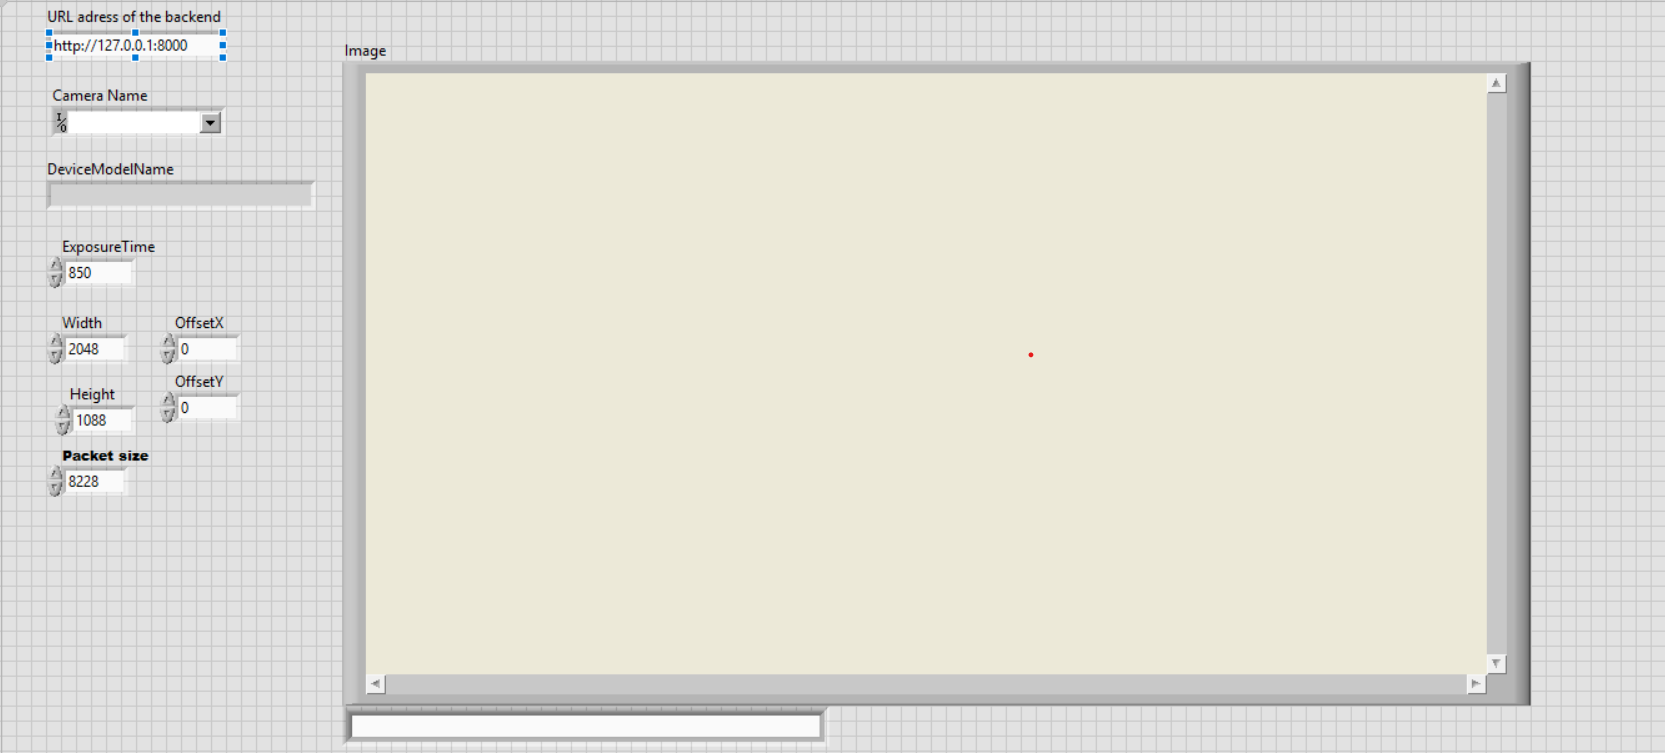
\includegraphics[width=0.95\textwidth]{../../img/labview-hyperspectral-cam-settings}
            \caption{Parametry MS v LabVIEW}
            \label{fig:params_ms_labview}
        \end{figure}

        \begin{itemize}
            \item \textbf{URL address of the backend} - adresa BE, kam LabVIEW bude posílat GET dotaz
            \item \textbf{Path} – cesta k obrázku, který pořídí kamera
            \item \textbf{CameraName} – musí být vybrána připojená MS
            \item \textbf{Width \& Height} – musí odpovídat hodnotám, které jsou v DeviceModelName (zde například D2048x1088)
            \item \textbf{Packet size} – musí být nastaven na hodnotu \textbf{8228}
        \end{itemize}

        Teprve teď můžeme spustit LabVIEW kód a FastAPI aplikaci v \texttt{labview-control/}.
        LabVIEW bude každou sekundu vysílat HTTP GET dotaz a pokud dostane hodnotu \texttt{1}, tak se pořídí snímek, jinak čeká.
        Dotaz je vysílán na FastAPI aplikaci.
    \end{teamwork}
\end{document}
